\documentclass[]{beamer}

\usepackage{beamerthemesplit}
\usepackage[utf8]{inputenc}
\usepackage[danish]{babel}
\usepackage[T1]{fontenc}
\usepackage{graphicx}
\usepackage{amsmath}
\usepackage{hyperref}
\usepackage{enumerate}
\usepackage{url}

\setbeamertemplate{navigation symbols}{} 
\useoutertheme{infolines} 
\setbeamercovered{transparent=40} 

\title{1. Seminar EVU RegAut}
\author[S. Meldgaard]{Sigurd Meldgaard\\
Ph.d. studerende i Kryptologi og Programmeringssprog}
\date{??. ?? 2010}
\institute[AU]{Datalogisk Institut\\
  Århus Universitet\\
  \texttt{stm@cs.au.dk}
}

\AtBeginSection[]
{
   \begin{frame}
       \frametitle{Plan}
       \tableofcontents[currentsection]
   \end{frame}
}

\begin{document}
%\begin{frame}[plain]
%  \titlepage
%\end{frame}
\maketitle
\begin{frame}
\frametitle{Plan}

\begin{itemize}[<alert@+>]
\item Hvad er Regularitet og Automater
\item Praktiske oplysninger om kurset
\item Regulære udtryk
\item Induktionsbevis
\item Frokost
\item Endelige automater
\item Skelnelighed, Produktkonstruktion
\item Præsentation af Java projekt
  \end{itemize}
\end{frame}

\section{Introduktion}

\begin{frame}
  \frametitle{Hvad er formålet med Regularitet og Automater?}
  \begin{itemize}[<+->]
  \item At præsentere matematiske teknikker og centrale begreber, der anvendes i datalogi
    \begin{itemize}
    \item Rekursive definitioner, induktionsbeviser
    \item Formelle sprog
    \item Modeller for beregnelighed
    \item Regularitet (``egenskaber som generelt kendetegner beregningsprocesser i it-systemer med begrænset mange tilstande'')    
    \end{itemize}
  \item Fundament for andre kurser
    \begin{itemize}
    \item Logik og Beregnelighed
    \item Oversættelse, 
    \item Sprog og Semantik
    \item Søgning og Optimering, ...
    \end{itemize}
  \end{itemize}
\end{frame}

\begin{frame}
\frametitle{Tekstgenkendelse}
\begin{itemize}
\item Specificere og genkende tekststrenge
\item søgning i tekster (Unix grep)
\item leksikalsk analyse i oversættere (flex)
\item HTML input validering (PowerForms)
\item ...
\item  
\item Konkret anvendelse af regulære udtryk og endelige automater

\end{itemize}
\end{frame}

\begin{frame}
\frametitle{Eksempel...}
\begin{center}
    \scalebox{0.35}{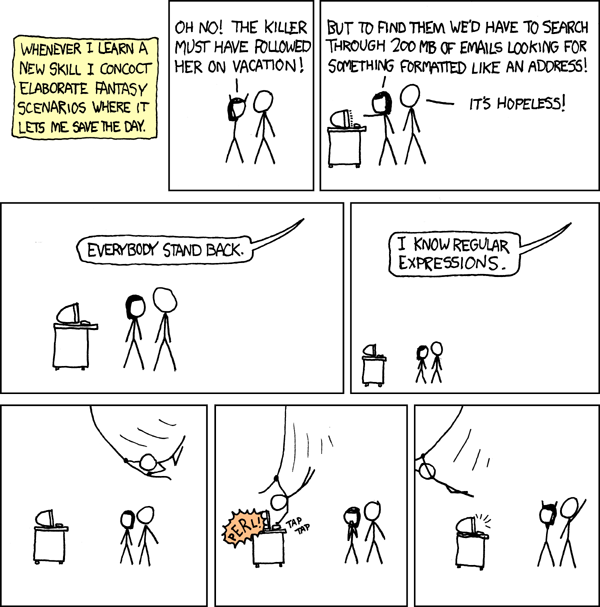
\includegraphics{images/xkcd}}
\end{center}
\end{frame}

\begin{frame}
  \frametitle{Eks. HTML formularer}
  HTML formularer indeholder input-felter, hvor
  brugeren kan indtaste tekststrenge.

  \begin{columns}
    \begin{column}{0.5\textwidth}
      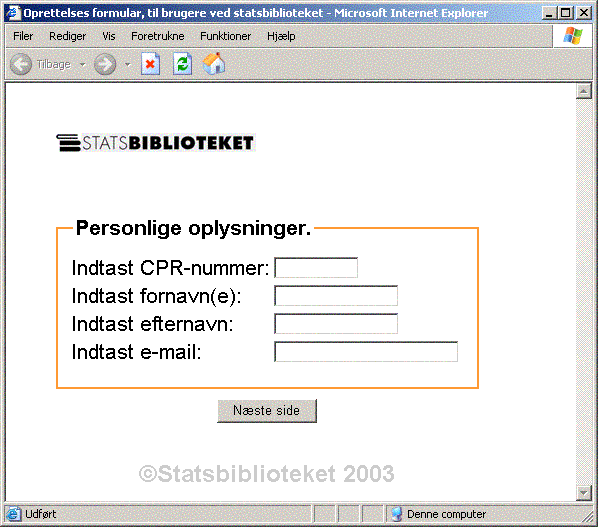
\includegraphics[width=\textwidth]{images/biblio}
    \end{column}

    \begin{column}{0.5\textwidth}
      For eksempel
      \begin{itemize}
      \item datoer
      \item telefonnumre
      \item CPR-numre
      \item emailadresser
      \item URL’er
      \item ...
      \end{itemize}
    \end{column}
\end{columns}

\end{frame}

\begin{frame}
\frametitle{HTML input valdidering}
\begin{itemize}[<+->]
\item Brugeren må ikke indtaste ugyldige strenge

\item Den traditionelle løsning: Programmer input validering i
JavaScript (til browseren – så input valideres løbende mens formularen udfyldes), og
Java (til serveren – for det tilfælde at browseren ikke udfører JavaScript-koden)
\item Problemer:
\begin{itemize}
\item Det er svært at programmere JavaScript, der virker på alle (nyere) browsere 
\item Vi skal skrive den samme kode i to forskellige sprog 
\item Store dele af koden skal skrives igen og igen...     
\end{itemize}
\end{itemize}
\end{frame}

\begin{frame}
\frametitle{Den datalogiske løsning}
\begin{itemize}[<+->]
\item Analysér problemområdet
\item Design et domæne-specifikt højniveau sprog
\item Lav en oversætter, der genererer JavaScript- og Java-koden fra højniveau specifikationer
\end{itemize}

Sproget \emph{PowerForms} er udviklet efter denne metode

Input-felter beskrives med \emph{regulære udtryk}, der oversættes til \emph{endelige automater}
\end{frame}
\section{Regulære udtryk}
\begin{frame}
\frametitle{Grundliggende begreber}
Vi starter med nogle \emph{matematiske definitioner}
\begin{itemize}[<+->]
\item Et \emph{alfabet} er en endelig mængde af tegn
\begin{itemize}
    \item Ex. $\{a,b,c,...z\}$
    \item Ex. ASCII, Unicode
    \item Ex. $\{0, 1\}$
\end{itemize}
\item En \emph{streng} er en endelig sekvens af tegn fra alfabetet
\begin{itemize}
    \item Ex. \texttt{"onkel sune drejer den usle kno"}
    \item Ex. \texttt{"10110"}
    \item Ex. \texttt{"\,"}  (Den tomme streng. Skrives også $\Lambda$).
\end{itemize}
\item Et \emph{sprog} er en mængde af strenge
\begin{itemize}
\item Ex. \texttt{\{"hans", "ole"\}}
\item Ex. $\{\Lambda, a, aa, aaa, aaaa, ...\}$
\item Ex. $\{\}$ (Det tomme sprog)
\item Ex. Alle korrekte danske sætninger
\end{itemize}
\end{itemize}
\end{frame}

\begin{frame}
\frametitle{Regulære udtryk}
Et \emph{regulært udtryk} beskriver et \emph{sprog}
\begin{itemize}
\item Regulære udtryk findes på 6 former
\item 3 basis-tilfælde:
\item $\emptyset$  	– den tomme mængde af strenge
\item $\Lambda$  	– mængden bestående af den tomme streng
\item $a\in\Sigma$	– mængden bestående af en enkelt streng, som
        	   er det ene tegn $a$ fra alfabetet $\Sigma$
\item Og 3 Sammensatte tilfælde (rekursive tilfælde):
\item $r_1+r_2$	– de strenge der beskrives af $r_1$ eller $r_2$
\item $r_1\dot r_2$	– de strenge der kan opdeles i to dele, så 
 	   venstre del beskrives af $r_1$ og højre del af $r_2$
\item $r^*$	– de strenge der kan opdeles i et antal dele,
		   der hver beskrives af $r$
\end{itemize}
\end{frame}
\end{document}
